{
\usebackgroundtemplate{\tikz\node[opacity=0.07,inner sep=0] {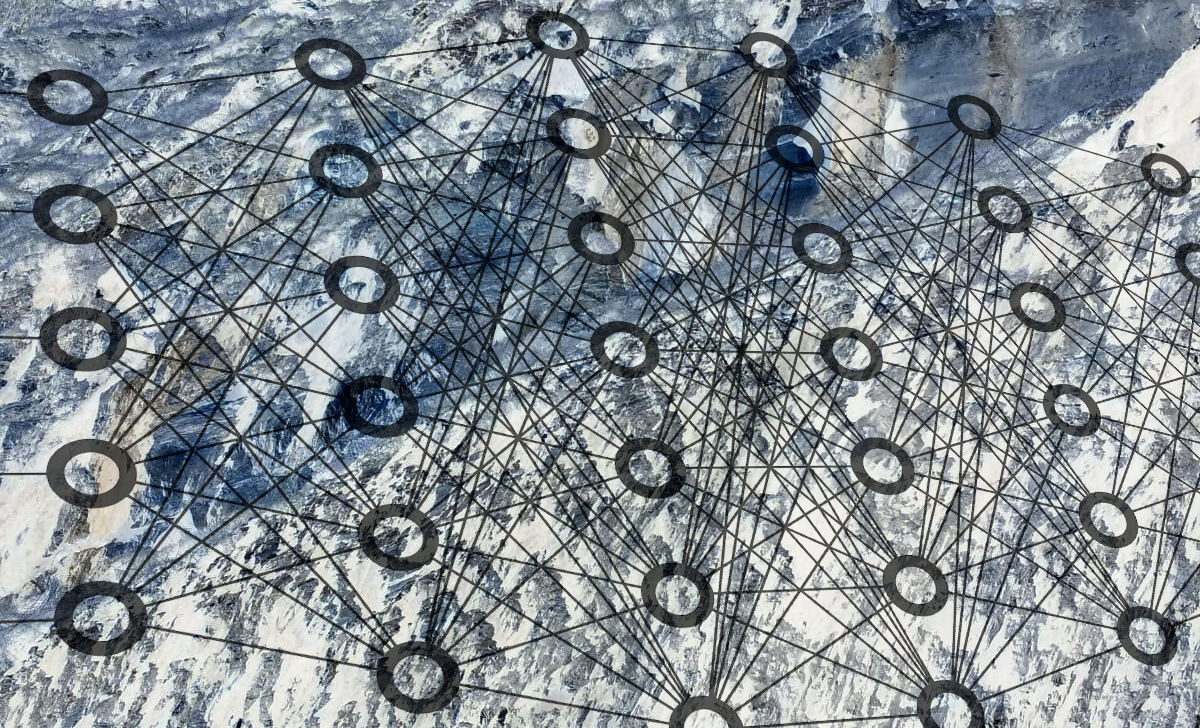
\includegraphics[height=\paperheight,width=\paperwidth]{frames/auxiliar/title_img/prueba.png}};}

\begin{frame}{Outline}
\begin{columns}
\begin{column}{0.05\textwidth}
\end{column}
\begin{column}{0.95\textwidth}

\mybullet{1}{Why Use Deep Learning?}

\vspace{0.4cm}

\mybullet{2}{Deep Learning for Solving Inverse and Forward Problems}

\vspace{0.4cm}

\mybullet{3}{Database Generation using rIGA}
%	\vspace{-0.2cm}
%	\begin{itemize}\setlength{\itemindent}{1cm}
%	\item Existing methods
%	\item Limitation for geophysical problems
%	\item Challenges: Integration, and Minimization
%	\end{itemize}

\vspace{0.4cm}

\mybullet{4}{Solving Forward Problems (PDEs) with Neural Networks}
%	\vspace{-0.2cm}
%	\begin{itemize}\setlength{\itemindent}{1cm}
%	\item Deep Finite Element Method
%	\item $r-$adaptivity with Deep Learning
%	\item Building the Riesz Operator with Deep Methods
%	\item Deep Fourier Method
%\end{itemize}


\vspace{0.4cm}

\mybullet{5}{Achievements}

\vspace{0.4cm}

\mybullet{6}{Conclusions and Future Work}
\end{column}
\end{columns}

\end{frame} 
}